%%%%%%%%%%%%%%%%%%%%%%%%%%%%%%%%%%%%%%%%%
% Hosei University Master's Thesis Template
% LaTeX Template
% Version 1.0 (15/05/2025)
% 
% 
% This template is based on the template by:
% Steve Gunn (http://users.ecs.soton.ac.uk/srg/softwaretools/document/templates/)
% Sunil Patel (http://www.sunilpatel.co.uk/thesis-template/)
% Johannes Böttcher (http://www.latextemplates.com/template/masters-doctoral-thesis)
% University of Hong Kong Masters/Doctoral Thesis (https://www.overleaf.com/latex/templates/hku-master-slash-doctoral-thesis-template/fstdrzngtktt)
% 
%
% Template license:
% CC BY-NC-ND 4.0 (https://creativecommons.org/licenses/by-nc-nd/4.0/)
%
% Author:  Zihan ZHAO
% Contact: zihan.zhao.4t@stu.hosei.ac.jp
%
%%%%%%%%%%%%%%%%%%%%%%%%%%%%%%%%%%%%%%%%%


%----------------------------------------------------------------------------------------
%	PACKAGES AND OTHER DOCUMENT CONFIGURATIONS
%----------------------------------------------------------------------------------------

\documentclass[hyphens,
10pt, % The default document font size, options: 10pt, 11pt, 12pt
%oneside, % Two side (alternating margins) for binding by default, uncomment to switch to one side
english, % ngerman for German
onehalfspacing, % Single line spacing (singlespacing), alternatives: onehalfspacing or doublespacing
% draft, % Uncomment to enable draft mode (no pictures, no links, overfull hboxes indicated)
% nolistspacing, % If the document is onehalfspacing or doublespacing, uncomment this to set spacing in lists to single
liststotoc, % Uncomment to add the list of figures/tables/etc to the table of contents
%toctotoc, % Uncomment to add the main table of contents to the table of contents
parskip, % Uncomment to add space between paragraphs
%nohyperref, % Uncomment to not load the hyperref package
headsepline, % Uncomment to get a line under the header
%chapterinoneline, % Uncomment to place the chapter title next to the number on one line
% consistentlayout, % Uncomment to change the layout of the declaration, abstract and acknowledgements pages to match the default layout
]{HoseiThesis} % The class file specifying the document structure

\RequirePackage{xcolor}
\usepackage[utf8]{inputenc} % Required for inputting international characters
\usepackage[T1]{fontenc} % Output font encoding for international characters
\usepackage{fontawesome} % Awesome symbol for usage
\usepackage{wrapfig} % Add enbedded figure in the text
\usepackage{tikz} % Add the signature figure overlap the text
% \usepackage[labelformat=simple]{subcaption} % Add multiple subfigures in a figure environment
% \captionsetup{justification=justified, margin=0pt}
% \renewcommand\thesubfigure{(\Alph{subfigure})} % change the image numbering and reference link to (A),(B),(C), ...... format

\usepackage{mathpazo} % Use the Palatino font by default
% \usepackage[backend=bibtex,style=alphabetic,natbib=true]{biblatex} % Use the bibtex backend with the authoryear citation style (which resembles APA)
\usepackage[
natbib=true,
maxbibnames=99,
giveninits=true,
style=ieee,
backend=biber
]{biblatex}
\defbibheading{Bibliography}{
  \section*{References}
  \markboth{References}{References}
}

\addbibresource{thesis.bib} % The filename of the bibliography
\addbibresource{bibs/Chapter1.bib}
\addbibresource{bibs/Chapter2.bib}
\addbibresource{bibs/Chapter3.bib}
\addbibresource{bibs/Chapter4.bib}

\usepackage[autostyle=true]{csquotes} % Required to generate language-dependent quotes in the bibliography

\AtBeginEnvironment{enquote}{\itshape} % change the quote words to italics style

\usepackage{rotating} % Required to add rotated big tables

\usepackage[normalem]{ulem} % Required to add dashed underlines

\setlength\parindent{2em}
%----------------------------------------------------------------------------------------
%	MARGIN SETTINGS
%----------------------------------------------------------------------------------------

\geometry{
	paper=a4paper, % Change to letterpaper for US letter
	left=3.5cm, % Left margin
	right=3.5cm, % Right margin
	bindingoffset=.5cm, % Binding offset
	top=2.5cm, % Top margin
	bottom=2.5cm, % Bottom margin
	%showframe, % Uncomment to show how the type block is set on the page
}

\usepackage{microtype}            % 启用微排版
\usepackage{adjustbox}
\usepackage{subcaption}
\usepackage{graphicx}
\usepackage{rotating}

\makeatletter
% 在 \begin{document} 时,把 emergencystretch 设为 0.1 倍的 \linewidth
\AtBeginDocument{%
  \setlength\emergencystretch{0.1\linewidth}%
  \hfuzz=1pt       % 允许最多 1pt 的小空隙不报错
  \hbadness=10000   % 阈值以下的不再警告 underfull hbox
}
\makeatother

% 可选:全局放宽换行惩罚
\sloppy


% \usepackage{microtype}            % 启用微排版增强
% \setlength\emergencystretch{1em}   % 在必要时允许每行多拉 1em 的额外空隙
% \sloppy

\setcounter{secnumdepth}{3}
\setcounter{tocdepth}{3}

%----------------------------------------------------------------------------------------
%	THESIS INFORMATION
%----------------------------------------------------------------------------------------

\thesistitle{Your Master Thesis Title}
% Thesis title, this is used in the title and abstract, print it elsewhere with \ttitle

\supervisor{Prof. Keping \textsc{Yu}}
\studentid{Your student id here}
% Your supervisor's name, this is used in the title page, print it elsewhere with \supname

% \cosupervisor{Prof. Keping \textsc{FamilyName}}
% Your supervisor's name, this is used in the title page, print it elsewhere with \supname
% \cosupervisor{Prof. Hayden K.-H. \textsc{So}} % Your supervisor's name, this is used in the title page, print it elsewhere with \cosupname

\examiner{}
% Your examiner's name, this is not currently used anywhere in the template, print it elsewhere with \examname

\degree{Master of Engineering (Applied Informatics)}
% Your degree name, this is used in the title page and abstract, print it elsewhere with \degreename

\author{Your firstname \textsc{Your Lastname}}
% The author name, this is used in the title page and abstract, print it elsewhere with \authorname

\addresses{}
% Your address, this is not currently used anywhere in the template, print it elsewhere with \addressname

\subject{Natural Language Processing}
% Your subject area, this is not currently used anywhere in the template, print it elsewhere with \subjectname

\keywords{Light field, high-dimensional convolutional neural network, deep learning}
% Keywords for your thesis, this is not currently used anywhere in the template, print it elsewhere with \keywordnames

\university{Hosei University}
% Your University's name and URL, this is used in the cover page and abstract, print it elsewhere with \univname

\bsuniversity{Hosei University}
\msuniversity{Hosei University}
% Your Bachelor/Master University's name and URL, this is used in the title page and abstract, print it elsewhere with \univname

\department{Major in Applied Informatics}
% Your department's name and URL, this is used in the title page and abstract, print it elsewhere with \deptname

\group{Laboratory of The Student}
% Your research group's name and URL, this is used in the title page, print it elsewhere with \groupname

\faculty{Graduate School of Science and Engineering}
% Your faculty's name and URL, this is used in the title page and abstract, print it elsewhere with \facname

\AtBeginDocument{
\hypersetup{pdftitle=\ttitle} % Set the PDF's title to your title
\hypersetup{pdfauthor=\authorname} % Set the PDF's author to your name
\hypersetup{pdfkeywords=\keywordnames} % Set the PDF's keywords to your keywords

\hypersetup{
  colorlinks,
  linkcolor=darkred,   % 交叉引用(目录、figure/table)保留 darkred
  urlcolor=darkred,    % URL 链接保留 darkred
  citecolor=darkred    % 文献引用也保留 darkred
}
}

\RenewDocumentCommand{\darkred}{m}{\textbf{#1}}
% \AtBeginEnvironment{algorithm}{\setstretch{2}}
\setlength{\algomargin}{1.3ex}


%----------------------------------------------------------------------------------------
%	NEW COMMAND DEFINITION
%----------------------------------------------------------------------------------------
\newcommand{\codestyle}[1]{\colorbox{gray!20}{\darkred{#1}}}

% ======================================================================================== %
%                                        START DOCUMENT
% ======================================================================================== %

\begin{document}

% \frontmatter % Use roman page numbering style (i, ii, iii, iv...) for the pre-content pages
\pagestyle{plain} % Default to the plain heading style until the thesis style is called for the body content


%----------------------------------------------------------------------------------------
%	COVER
%----------------------------------------------------------------------------------------

\begin{titlepage}
\addtocounter{page}{-1}
\begin{center}

\vspace*{.024\textheight}
% \begin{tabular}{c}
%     % 
\includegraphics[align=c, width=0.18\textwidth]{Covers/logo.png} &  
%     \scshape \huge \univname % University name
% \end{tabular}

\vspace{1cm}
% \textsc{\Large Master's Thesis}\\[0.5cm] % Thesis type


% \rule[0.4cm]{13cm}{0.1pt}\\% \HRule \\[0.4cm] % Horizontal line
{\huge \bfseries \ttitle\par}\vspace{4cm} % Thesis title
% \HRule \\[1.5cm] % Horizontal line
% \rule{13cm}{0.1pt}\\ \vspace{1.5cm}
 
% \begin{minipage}[t]{0.4\textwidth}
% \begin{flushleft} \large
% \emph{Author:}\\
% \authorname % Author name - remove the \href bracket to remove the link
% \end{flushleft}
% \end{minipage}
% \begin{minipage}[t]{0.4\textwidth}
% \begin{flushright} \large
% \emph{Supervisor:} \\
% \supname \\ % Supervisor name - remove the \href bracket to remove the link
% % \emph{Co-Supervisor:} \\
% % \href{https://kenkyu-web.hosei.ac.jp/hosei/detail.html?systemId=e29d8dfb67b36866&lang=en}{\cosupname} % Supervisor name - remove the \href bracket to remove the link 
% \end{flushright}
% \end{minipage}\\[1.6cm]
 
\vfill

\large \textit{A Dissertation\\Presented to Institute of Integrated Science and Technology (IIST)}\\[0.4cm] % University requirement text \degreename
\textit{by}\\[0.4cm]
\authorname \\
\stuid \\[2.5cm]
% \groupname\\
In Partial Fulfillment\\of the Requirements for the Master Degree,\\
\deptname \\
\facname, \textsc{Hosei University} \\[1.6cm] % Research group name and department name
 
\vfill

Supervisor: \supname \\[0.5cm]
\textsc{Hosei University}\\
\number\year \; Master Thesis
% {\large \usdate\today}\\[4cm] % Date
%\includegraphics{Logo} % University/department logo - uncomment to place it
 
\vfill
\end{center}

\end{titlepage}


% \blankpage
% \addtocounter{page}{-1}

%----------------------------------------------------------------------------------------
%	COPYRIGHT PAGE
%----------------------------------------------------------------------------------------

\newpage
\thispagestyle{empty}
\addtocounter{page}{-1}

\vspace*{\fill}
\scshape \noindent Copyright \copyright 2025, by \authorname \\
\noindent all rights reserved.
\vspace*{\fill}
\newpage
\rm


\frontmatter
\tableofcontents % Prints the main table of contents


%----------------------------------------------------------------------------------------
%	ABSTRACT PAGE
%----------------------------------------------------------------------------------------
\mainmatter
\pagestyle{thesis} % Return the page headers back to the "thesis" style

% \begin{abstract}
% \addchaptertocentry{\abstractname} % Add the abstract to the table of contents
% Put Your \emph{Abstract} Here ...
% \tableofcontents


% \mainmatter
% \pagenumbering{arabic}
% \setcounter{page}{1}
\chapter*{Abstract}
\addchaptertocentry{Abstract}

Your abstract here.....


% \end{abstract}


%----------------------------------------------------------------------------------------
%	TITLE PAGE
%----------------------------------------------------------------------------------------
% \pagestyle{empty}
\newpage
\addtocounter{page}{-1}
\begin{center}
\vspace*{2cm}
\huge{ \bf \ttitle}
\end{center}

\vspace{20mm}
\begin{center}
by

\vspace{10mm}
{\bf \authorname}\\
M.Eng. \textit{\msunivname}
\end{center}

\vspace{30mm}
\begin{center}
A Thesis Submitted in Fulfilment \\
of the Requirements for the Degree of \\
\degreename \\
\vspace{10mm}
at \\
\vspace{10mm}
\univname\\
%February 2015
\monthyeardate\today
\end{center}




%----------------------------------------------------------------------------------------
%	DECLARATION PAGE
%----------------------------------------------------------------------------------------

% \begin{declaration}
\setcounter{page}{1}
\addchaptertocentry{\authorshipname} % Add the declaration to the table of contents

\vspace{0.6cm}
I, \authorname, declare that this thesis titled, \enquote{\ttitle}, which is submitted in fulfillment of the requirements for the Degree of Master of Engineering, represents my own work except where due acknowledgement have been made. I further declared that it has not been previously included in a thesis, dissertation, or report submitted to this University or to any other institution for a degree, diploma or other qualifications.


\vspace{2cm} 
\begin{flushright}
\hfill Signed: \underline{\hspace{5cm}}\\[2em] % This prints a line for the signature
\hfill Date: \underline{\hspace{1.5cm} \usdate\today \hspace{1.5cm}}\\ % This prints a line to write the date
\end{flushright}

% Signature
\begin{tikzpicture}[remember picture,overlay]
\node[xshift=-6cm,yshift=-18cm] at (current page.north east){%
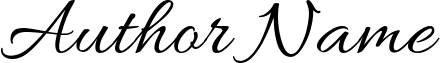
\includegraphics[width=3.6cm]{Figures/signature.png}};
\end{tikzpicture}
\end{declaration}





%----------------------------------------------------------------------------------------
%	QUOTATION PAGE
%----------------------------------------------------------------------------------------

% \begin{dedication}
\setcounter{page}{2}
\addchaptertocentry{\dedicationname} % Add the acknowledgements to the table of contents
\vspace{1cm}


\noindent I would like to thank...
\\[0.4cm]

% \hfill
\begin{flushright}
    \authorname \\
    Hosei University \\
    \usdate\today
\end{flushright}

\end{dedication}




%----------------------------------------------------------------------------------------
%	THESIS CONTENT - CHAPTERS
%----------------------------------------------------------------------------------------

% \mainmatter % Begin numeric (1,2,3...) page numbering



% Include the chapters of the thesis as separate files from the Chapters folder
% Uncomment the lines as you write the chapters

% Chapter 1

\chapter{Introduction} % Main chapter title

\label{Chapter1} % For referencing the chapter elsewhere, use \ref{Chapter1} 

%----------------------------------------------------------------------------------------

% Define some commands to keep the formatting separated from the content 
% \newcommand{\keyword}[1]{\textbf{#1}}
% \newcommand{\tabhead}[1]{\textbf{#1}}
% \newcommand{\code}[1]{\texttt{#1}}
% \newcommand{\file}[1]{\texttt{\bfseries#1}}
% \newcommand{\option}[1]{\texttt{\itshape#1}}

%----------------------------------------------------------------------------------------

% =========================================================== %
%                 Section: Problem Introductionn                %
% =========================================================== %
\section{Background and Motivation}
\label{chap1:sec1}


% =========================================================== %
%      Section: Main Contributions       %
% =========================================================== %
\section{Main Research Contributions}
\label{chap1:sec2}


% =========================================================== %
%      Section: Dissertation Outline       %
% =========================================================== %
\section{Organization of the Dissertation}
\label{chap1:sec3}

\chapter{Fundamentals of (Your research topic here)} 

\label{Chapter2} 
% Chapter 3

\chapter{Experimental Configuration and Preliminaries}
\label{Chapter3} 

This chapter provides a unified description of the uniformity of all the experimental environments, datasets, evaluation metrics, and baselines selected for your papers. If your research is based on the same dataset, you can, like me, dedicate a separate chapter to them. Otherwise, you can also write a preliminary description for each of the proposals you have made (each proposal corresponds to one of the methods below).

\chapter{Your method in type 1} 
\label{Chapter4}

This is the method you proposed.
\chapter{Your method in type 2} 
\label{Chapter4}

This is the 2nd method you proposed. 

One of friendly reminders is, if you have only one article, or if different articles address the same problem, please adjust whether a second methodology chapter is necessary based on the specific situation.
% Chapter 6

\chapter{Conclusion} 
\label{Chapter6} 

Your Conclusion here......

%----------------------------------------------------------------------------------------
%	THESIS CONTENT - APPENDICES
%----------------------------------------------------------------------------------------

% \chapter*{References}
% % References
% \addcontentsline{toc}{chapter}{References} 

%----------------------------------------------------------------------------------------
%	BIBLIOGRAPHY
%----------------------------------------------------------------------------------------



\printbibliography[title={References}, heading=bibintoc]


%----------------------------------------------------------------------------------------

%----------------------------------------------------------------------------------------
%	ACKNOWLEDGEMENTS
%----------------------------------------------------------------------------------------
% \begin{acknowledgements}
\chapter*{Acknowledgements}
% \setcounter{page}{2}
\addchaptertocentry{\acknowledgementname} % Add the acknowledgements to the table of contents
% \vspace{1cm}


\noindent I would like to thank...
\\[0.4cm]

% \hfill
\begin{flushright}
    \authorname \\
    Hosei University \\
    \usdate\today
\end{flushright}

% \end{acknowledgements}

%----------------------------------------------------------------------------------------
%	LIST OF PUBLICATIONS PAGES
%----------------------------------------------------------------------------------------


\begin{publications}
\addcontentsline{toc}{chapter}{List of Publications}
\newcommand{\JourConfTitle}[1]{\ul{\emph{#1}}}


% ---------------------------------------------------------------------------
% JOURNALS
% ---------------------------------------------------------------------------

\begin{journals}

\item Your journal paper here in IEEE Trans format...

\item Your journal paper here in IEEE Trans format...

% \item \textbf{Z. Zhao}, Y. Zhu, S. Zhang, C. Chakraborty, O. Alfarraj, A. Tolba, and K. Yu, “WMPA-ConvBERT-BM: A Enhanced Hybrid Deep Learning Model 
% for IoT-Enabled Malicious URLs Detection Tasks with Whale-Marine Predator Algorithm Optimization,” Internet of Things, 2025, Major revision compeleted, ISSN: 2542-6605. \textbf{(JCR Q1; IF=6.0)}

% \item C. Rong, J. Seo, \textbf{Z. Zhao}, F. Ö. Catak, J. Geng, and M. G. Jaatun, “Federated Large Domain Model System,” Blockchain: Research and Applications, 2025, ISSN: 2096-7209. DOI: 10.1016/j.bcra.2025.100277. [Online]. Available: https://doi.
% org/10.1016/j.bcra.2025.100277. \textbf{(JCR Q1; IF=6.9)}

\end{journals}

% \newpage
% ---------------------------------------------------------------------------
%  CONFERENCES
% ---------------------------------------------------------------------------

\begin{conferences}
\item Your conference paper here in IEEE Trans format...

\item Your conference paper here in IEEE Trans format...

% \item \textbf{Z. Zhao}, J. Chen, F. J. A. Messou, R. Katabarwa, and K. Yu, “A Resource-efficient Text-to-Text Transfer Transformer Encoder-based Vertical Hybrid Model for Malicious URLs Detection,” in 2024 IEEE 100th Vehicular Technology Conference (VTC2024-Fall), IEEE, 2024, pp. 1–6.

% \item Y. Zhu, \textbf{Z. Zhao}, S. Zhang, J. Sun, and K. Yu, “MauBa: A Multi-Agent Coordination Framework for Vision-Language-Guided Zero-Shot Control of Unmanned Aerial Vehicles,” in Submitted to the 2025 IEEE Global Communications Conference (GLOBECOM 2025), Under review, IEEE, 2025, pp. 1–5.

% \item J. Chen, \textbf{Z. Zhao}, F. J. A. Messou, R. Katabarwa, O. Alfarraj, K. Yu, and M. Guizani, “A Byzantine-Fault-Tolerant Federated Learning Method Using Tree-Decentralized Network and Knowledge Distillation for Internet of Vehicles,” in 2024 IEEE 100th Vehicular Technology Conference (VTC2024-Fall), IEEE, 2024, pp. 1–6.

% \item F. J. A. Messou, J. Chen, R. Katabarwa, \textbf{Z. Zhao}, and K. Yu, “Enhancing Short-Term Load Forecasting in Internet of Things: A Hybrid Attention-based CNN-BiLSTM with Data Augmentation Approach,” in 2024 IEEE 100th Vehicular Technology Conference (VTC2024-Fall), IEEE, 2024, pp. 1–6.

% \item J. Chen, \textbf{Z. Zhao}, K. Yu, S. Mumtaz, J. J. Rodrigues, M. Guizani, and T. Sato, “Enhancing Production Planning in the Internet of Vehicles: A Transformer-based Federated Reinforcement Learning Approach,” in 2024 IEEE 99th Vehicular Technology Conference (VTC2024-Spring), IEEE, 2024, pp. 1–6.
\end{conferences}



% Among the above-mentioned published papers, those published as the first author
% (Zihan Zhao) are related to this master's thesis research.

\end{publications}


%----------------------------------------------------------------------------------------
%	LIST OF CONTENTS/FIGURES/TABLES PAGES
%----------------------------------------------------------------------------------------



% \listoffigures % Prints the list of figures

% \listoftables % Prints the list of tables

% \listofalgorithms % Prints the list of algorithms
% \addchaptertocentry{\listalgorithmcfname}
%----------------------------------------------------------------------------------------
%	ABBREVIATIONS
%----------------------------------------------------------------------------------------
% \begin{abbreviations}{ll} % Include a list of abbreviations (a table of two columns)

\textbf{ASAP} & \textbf{A}s \textbf{S}oon \textbf{A}s \textbf{P}ossible \\
\textbf{AKA} & \textbf{A}lso \textbf{K}nown \textbf{A}s \\
\textbf{BPFA} & \textbf{B}eta \textbf{P}rocess \textbf{F}actor \textbf{A}nalysis \\
\textbf{CNN} & \textbf{C}onvolutional \textbf{N}eural \textbf{N}etwork \\
\textbf{GAN} & \textbf{G}enerative \textbf{A}dversarial \textbf{N}etwork \\
\textbf{MSE} & \textbf{M}ean \textbf{S}quare \textbf{E}rror \\
\textbf{PSNR} & \textbf{P}eak \textbf{S}ignal-to-\textbf{N}oise \textbf{R}atio \\
\textbf{SSIM} & \textbf{S}tructural \textbf{SIM}ilarity \\

\end{abbreviations}


%----------------------------------------------------------------------------------------
%	SYMBOLS
%----------------------------------------------------------------------------------------
% \begin{symbols}{p{0.15\textwidth}p{0.7\textwidth}l} % Include a list of Symbols (a three column table)

\multicolumn{3}{l}{\symboltitle{Global notations}}\\ \\
$I^\mathrm{SR}$ & super-resolved light field image & --- \\
$I^\mathrm{LR}$ & low-resolution light field image & --- \\
$I^\mathrm{HR}$ & high-resolution light field image & --- \\
$E^\mathrm{SR}$ & super-resolved epipolar plane image & --- \\
$E^\mathrm{HR}$ & high-resolution epipolar plane image & --- \\ \\
% $L$ & light field function & --- \\

\multicolumn{3}{l}{\symboltitle{Chapter~1}}\\ \\
$\theta$, $\phi$ & incoming direction expressed in term of spherical coordinates & rad \\
$\tau$ & time & s (second)\\
$x$,$y$ & spatial coordinates with two-plane parameterization & 1 (uint) \\
$s$,$t$ & angular coordinates with two-plane parameterization & 1 (uint) \\
$P$ & radiance distribution & \si{\watt\per\steradian \square{\metre} \text{\hertz}} \\
$\Omega$ & image plane & --- \\
$\Theta$ & parameters of the multi-layer framework & --- \\
$\gamma_s$, $\gamma_a$ & scaling factors of spatial / angular coordinates & 1 (uint) \\
$\mathcal{L}$ & loss function & --- \\ \\

\multicolumn{3}{l}{\symboltitle{Chapter~2}}\\ \\
$F_0$ & shallow features extracted by a single HConv layer & --- \\
$F_\mathrm{G_d}$ & feature maps extracted by the $d^\mathrm{th}$ HRB of the GRLNet & --- \\
$H_\mathrm{HRB}^\mathrm{n}$ & the operation of the $n^\mathrm{th}$ HRB of the SReNet & --- \\
$H_\mathrm{AGBN}$ & the operation of the proposed aperture group batch normalization algorithm & --- \\
$H_\mathrm{up}$ & upsampling operation on the low-resolution features & --- \\ \\


$\ell_A$ & angular loss & --- \\
$\ell_S$ & spatial perceptual loss & --- \\ 
$\ell_{SA}$ & the weighted combination of $\ell_A$ and $\ell_S$& --- \\
$f$ & the summation of all the feature maps after every activation function of VGG network & --- \\
$g$ & learned mapping between the low-resolution and high-resolution light field images & --- \\ \\


\multicolumn{3}{l}{\symboltitle{Chapter~3}}\\ \\
$x$,$y$ & spatial coordinates with two-plane parameterization & 1 (uint) \\
$s$,$t$ & angular coordinates with two-plane parameterization & 1 (uint) \\
$\gamma_s$, $\gamma_a$ & scaling factors of spatial / angular coordinates & 1 (uint) \\
$\ell_G$ & generator adversarial loss & --- \\
$\phi$ & denotes the mapping of VGG network & --- \\
$\delta$ & nearest neighbor downsampling operator & --- \\
$\kappa$ & a Gaussian blurring kernel with a window size of $7 \times 7$ and standard deviation of 1.2 pixels & --- \\
$\eta$ & additive noise with zero mean and unit standard deviation & --- \\ \\

\end{symbols}



\appendix % Cue to tell LaTeX that the following "chapters" are Appendices

% Include the appendices of the thesis as separate files from the Appendices folder
% Uncomment the lines as you write the Appendices

% % Appendix A

\chapter{About Appendix} % Main appendix title
\label{AppendixA} % For referencing this appendix elsewhere, use \ref{AppendixA}
The appendix is usually used to provide some supplementary materials for the publications. For example, some experimental results, network architecture, detailed experimental settings or proving of the theories. You can have more than one appendices to provide the materials for different uses.

% % Appendix Template

\chapter{Appendix Title Here} % Main appendix title

\label{AppendixX} % Change X to a consecutive letter; for referencing this appendix elsewhere, use \ref{AppendixX}

Write your Appendix content here.
% % Appendix Template

\chapter{Appendix Title Here} % Main appendix title

\label{AppendixX} % Change X to a consecutive letter; for referencing this appendix elsewhere, use \ref{AppendixX}

Write your Appendix content here.

%----------------------------------------------------------------------------------------

\end{document}
